
%(BEGIN_QUESTION)
% Copyright 2011, Tony R. Kuphaldt, released under the Creative Commons Attribution License (v 1.0)
% This means you may do almost anything with this work of mine, so long as you give me proper credit

This diesel engine-generator system provides electricity to power a small town during emergencies.  The engine, however, is not powerful enough to supply the maximum electrical load of the town, and may overheat if pressed into continuous service under maximum-load conditions:

$$\includegraphics[width=15.5cm]{i02427x01.eps}$$

Examine this control system diagram, then explain in your own words how it is supposed to work.  Propose a ``thought experiment'' where you can explore the system's operation under normal as well as overload conditions.

\vskip 20pt \vbox{\hrule \hbox{\strut \vrule{} {\bf Suggestions for Socratic discussion} \vrule} \hrule}

\begin{itemize}
\item{} A problem-solving technique useful for analyzing control systems is to mark the PV and SP inputs of all controllers with ``+'' and ``$-$'' symbols, rather than merely label each controller as ``direct'' or ``reverse'' action.  Apply this technique to the control strategy shown here, identifying which controller input(s) should be labeled ``+'' and which controller input(s) should be labeled ``$-$''.
\item{} Identify at least one instrument fault that would essentially shut the generator down, calling for zero output power from the diesel engine.
\end{itemize}

\underbar{file i02427}
%(END_QUESTION)





%(BEGIN_ANSWER)

Under normal conditions, the engine's power output is regulated by the voltage controller (EIC).  However, if engine temperature ever exceeds the safe operating setpoint, the temperature controller (TIC) overrides the voltage controller by calling for reduced engine power.  The low-select function selects which ever controller is calling for the {\it least} amount of engine power.

\vskip 10pt

Either a failed-high temperature transmitter or a failed-high voltage transmitter would call for zero power output by the engine.

%(END_ANSWER)





%(BEGIN_NOTES)


%INDEX% Control, strategies: override control
%INDEX% Process: diesel engine generator system

%(END_NOTES)


